% Include from si.tex after report.py has generated and validated all five models.
\begin{figure}[p]
\centering
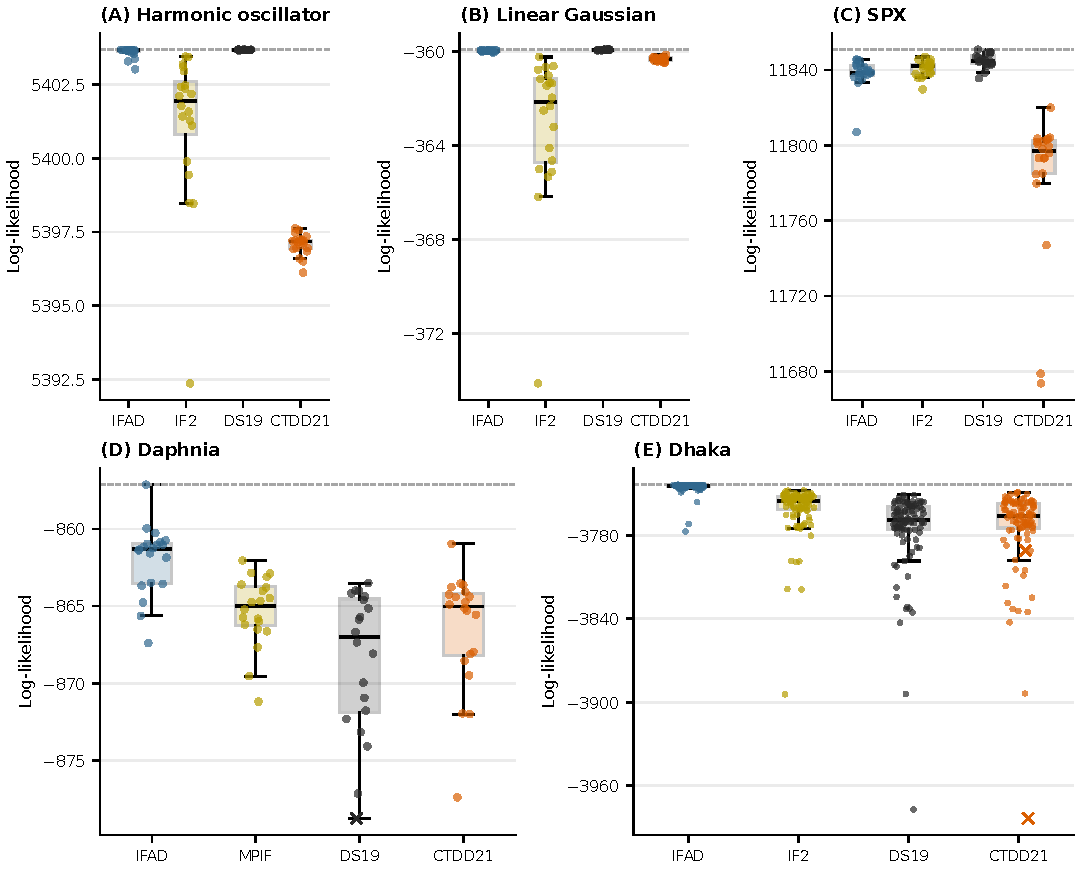
\includegraphics[width=\textwidth]{imgs/benchmarks/final_likelihoods.pdf}
\caption{Final log-likelihoods from repeated parameter searches.
Each point represents one of 20 searches per method in panels A--D
or 100 searches in panel E.
Boxes show the median and interquartile range; whiskers extend to the most
extreme values within 1.5 interquartile ranges of the box.
All estimates are shown, including those outside the whiskers.
Crosses mark searches that stopped prematurely, for which we evaluated
the last estimate obtained before failure or the time limit.
Dashed lines mark the analytic maximum in panels A and B
and the best displayed estimate in panels C--E.
Likelihoods are evaluated independently of fitting, using the same model
within each panel. All axes are linear.}
\label{fig:benchmark-final-likelihoods}
\end{figure}

\begin{figure}[p]
\centering
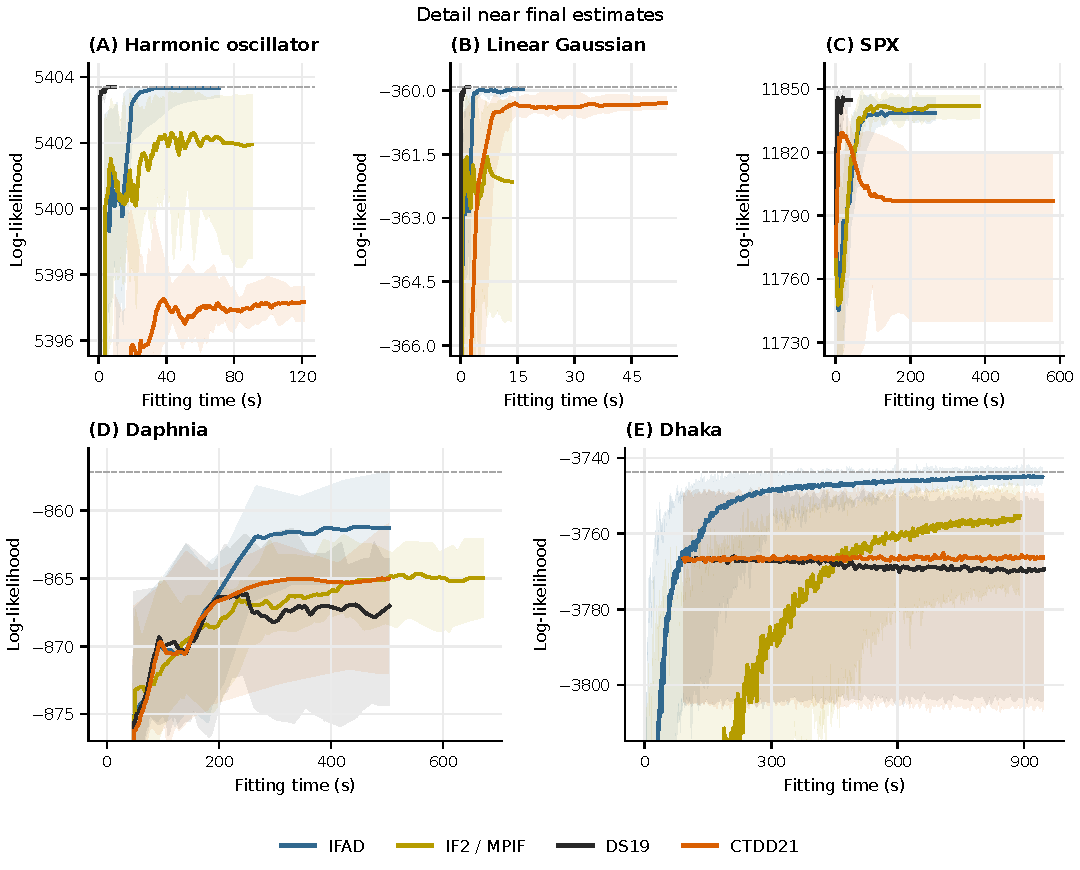
\includegraphics[width=\textwidth]{imgs/benchmarks/optimization_detail.pdf}
\caption{Optimization progress near the final estimates.
Solid lines show the median log-likelihoods, and the shaded regions cover
the area between the 10th and 100th percentiles across searches.
We evaluated likelihoods at saved iterations and interpolated linearly
between them, retaining each search's final value after it stopped.
These evaluations were not used to select the fitted parameters.
The vertical axes are linear and restricted to the region near the
final estimates; Figure~\ref{fig:benchmark-optimization-full} shows
the full range, with the same shading opacity.
The starting points, reference lines and final evaluations are those of
Figure~\ref{fig:benchmark-final-likelihoods}.}
\label{fig:benchmark-optimization-detail}
\end{figure}

\begin{figure}[p]
\centering
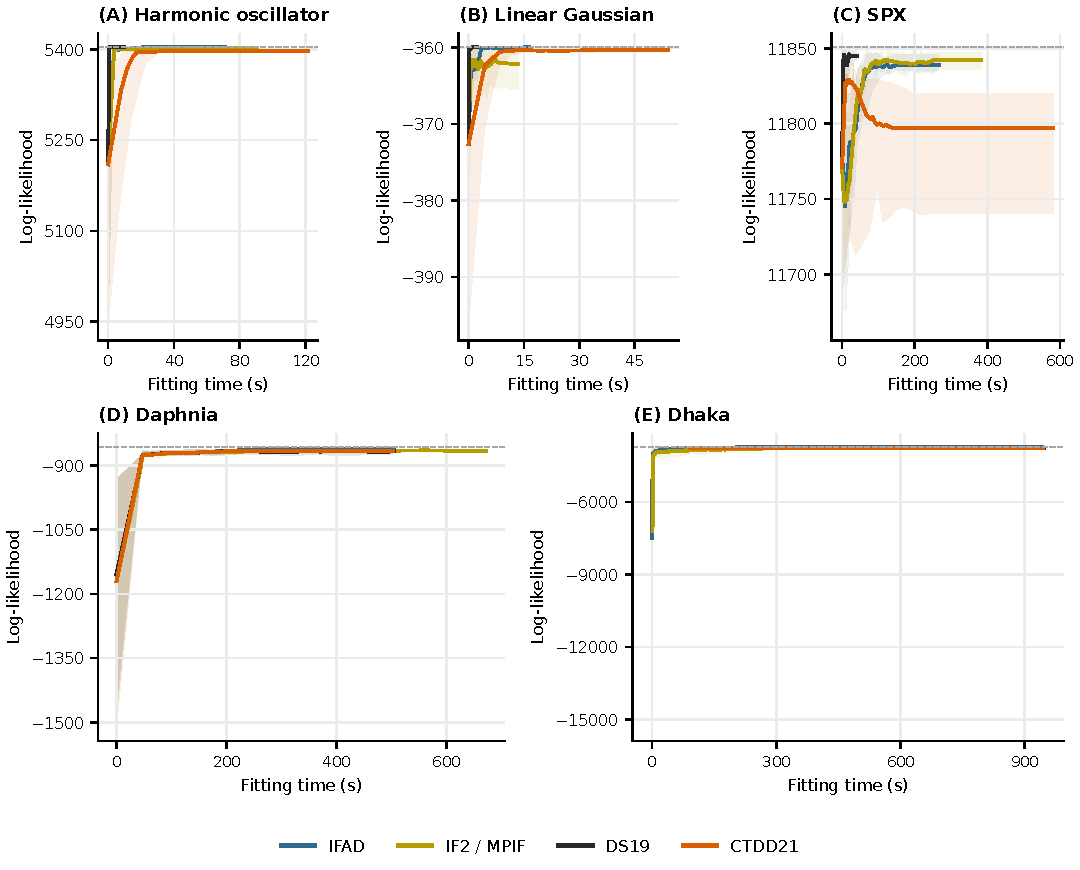
\includegraphics[width=\textwidth]{imgs/benchmarks/optimization.pdf}
\caption{Optimization progress over the full range of the median
trajectories and percentile bands. Lines, shading and reference lines are
defined in Figure~\ref{fig:benchmark-optimization-detail}.
All axes are linear, with separate ranges for each model and data set.
Computation times exclude compilation and independent likelihood
evaluation. The hardware and algorithmic settings are given in
Section~\ref{sec:benchmark-settings} and the preceding paragraph.}
\label{fig:benchmark-optimization-full}
\end{figure}

\begin{table}[p]
\centering
\small
\begin{tabular}{lrrrrrr}
\toprule
Method & Median & Maximum & IQR & MCSE & Time (s) & Failed \\
\midrule
\multicolumn{7}{l}{\textit{Harmonic oscillator (20 starts)}} \\
IFAD & 5403.67 & 5403.69 & 0.04 & 0.00 & 70.0 & 0 \\
IF2 & 5401.95 & 5403.46 & 1.80 & 0.00 & 89.4 & 0 \\
DS19 & 5403.69 & 5403.69 & 0.01 & 0.00 & 9.4 & 0 \\
CTDD21 & 5397.18 & 5397.63 & 0.28 & 0.00 & 117.3 & 0 \\
\addlinespace
\multicolumn{7}{l}{\textit{Linear Gaussian (20 starts)}} \\
IFAD & -359.96 & -359.94 & 0.03 & 0.00 & 16.1 & 0 \\
IF2 & -362.14 & -360.23 & 3.60 & 0.00 & 13.3 & 0 \\
DS19 & -359.93 & -359.92 & 0.01 & 0.00 & 2.1 & 0 \\
CTDD21 & -360.31 & -360.14 & 0.13 & 0.00 & 51.6 & 0 \\
\addlinespace
\multicolumn{7}{l}{\textit{SPX (20 starts)}} \\
IFAD & 11838.63 & 11845.69 & 4.95 & 0.31 & 144.5 & 0 \\
IF2 & 11841.96 & 11846.95 & 5.06 & 0.31 & 249.8 & 0 \\
DS19 & 11844.83 & 11850.85 & 4.11 & 0.47 & 21.5 & 0 \\
CTDD21 & 11796.97 & 11820.04 & 17.37 & 0.19 & 165.9 & 0 \\
\addlinespace
\multicolumn{7}{l}{\textit{Daphnia (20 starts)}} \\
IFAD & -861.30 & -857.13 & 2.57 & 0.19 & 487.8 & 0 \\
MPIF & -864.98 & -862.05 & 2.53 & 0.19 & 647.3 & 0 \\
DS19 & -867.02 & -863.52 & 7.37 & 0.20 & 488.1 & 1 \\
CTDD21 & -865.03 & -860.97 & 4.00 & 0.17 & 488.7 & 0 \\
\addlinespace
\multicolumn{7}{l}{\textit{Dhaka (100 starts)}} \\
IFAD & -3744.40 & -3743.68 & 0.95 & 0.14 & 942.8 & 0 \\
IF2 & -3755.41 & -3747.82 & 9.21 & 0.15 & 889.3 & 0 \\
DS19 & -3769.04 & -3751.03 & 16.53 & 0.17 & 942.8 & 0 \\
CTDD21 & -3765.91 & -3749.10 & 17.78 & 0.15 & 942.8 & 2 \\
\bottomrule
\end{tabular}

\caption{Repeated-search results for the five models.
Median, maximum and interquartile range (IQR) summarize final log-likelihoods
across searches. MCSE is the median Monte Carlo standard error of an
individual final log-likelihood estimate; it is zero for the analytic
Gaussian evaluations. Time is the median fitting time, including any IF2
or MPIF warm start and excluding compilation and independent evaluation.
Failed is the number of searches that stopped prematurely. We retained
their last estimates before failure or the time limit in all summaries.
Hardware and fitting settings differ
between experiments, as described in the text.}
\label{tab:benchmark-results}
\end{table}
